\documentclass[../main.tex]{subfiles}

\begin{document}

\section{Teljesítményváltozók}

\begin{fulltheorem}
  Ismertesse a következő fogalmakat!
  (adja meg a definícióját és rövid értelmezését)
  \begin{itemize}
    \item Extenzív és intenzív fizikai mennyiségek
    \item Átmenő és keresztváltozók
    \item Á, K és P típusú kétpólusok
    \item Csatolt kétpólus elem (transzformátor és girátor)
    \item Ideális kétpólusú források
  \end{itemize}
  Adja meg az Elektromos áramkör, Haladó és forgómozgású rendszer, Pneumatikus
  és Hidraulikai rendszer, valamint Termikus rendszer koncentrált paraméterű
  kétpólusú leírása esetén az átmenő és keresztváltozó típusát, valamint az Á,
  K és P típusú kétpólusok megnevezését (amennyiben léteznek).
\end{fulltheorem}

\subsection{Extenzív és intenziv fizikai mennyiségek}

Az \kix{intenzív fizikai mennyiség}[ek] a rendszer egyesítésére nézve
kiegyenlítődnek. Az általános elmozdulásmennyiség rátájának is nevezik őket.
Ilyen mennyiségek: hőmérséklet, nyomás, sűrűség, feszültség.

Az \kix{extenzív fizikai mennyiség}[ek] a rendszer egyesítésére nézve
additívak. Az általános impulzus rátájának is nevezik őket.
Megmaradási törvény rendelhető hozzájuk.
Ilyen mennyiségek: tömeg, térfogat, entrópia, töltés, energia.

\subsection{Átmenő és keresztváltozók}

A \kix{keresztváltozó}[k] az intenzív, míg az \kix{átmenő változó}[k]
az extenzív mennyiségekből származtathatóak. Szorzatuk a teljesítmény,
ezért \kix{teljesítményváltozó}[knak] is szokás őket nevezni.

\begin{figure}[H]
  \centering
  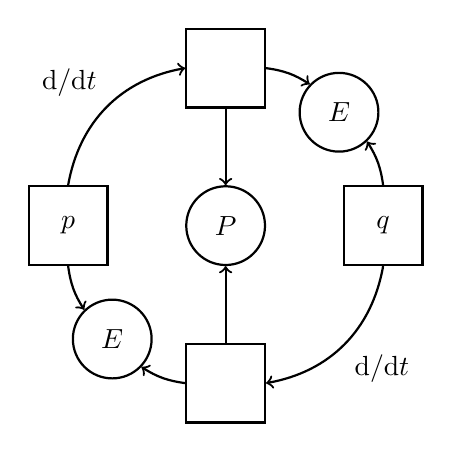
\begin{tikzpicture}[
      thick, scale=.8,
      rect/.style={rectangle, draw=black,minimum width=1cm, minimum height=1cm},
      circ/.style={circle, draw=black,minimum width=1cm, minimum height=1cm},
    ]
    \node[rect] (u) at (0,2.5) {$\varPhi$};
    \node[rect] (l) at (-2.5,0) {$p$};
    \node[rect] (r) at (2.5,0) {$q$};
    \node[rect] (d) at (0,-2.5) {$\itChi$};
    \node[circ] (m)  at (0,0) {$P$};
    \node[circ] (e1) at (-1.8,-1.8) {$E$};
    \node[circ] (e2)at (+1.8,+1.8) {$E$};

    \draw[-to] (u) -- (m);
    \draw[-to] (d) -- (m);
    \draw[-to] (l.north) to[bend left=35] node[midway, above left] {$\mathrm{d/d}t$} (u.west);
    \draw[-to] (r.south) to[bend left=35] node[midway, below right] {$\mathrm{d/d}t$} (d.east);
    \draw[-to] (d.west) to[bend left=12.5] (e1);
    \draw[-to] (l.south) to[bend right=12.5] (e1);
    \draw[-to] (u.east) to[bend left=12.5] (e2);
    \draw[-to] (r.north) to[bend right=12.5] (e2);
  \end{tikzpicture}
  \caption{A teljesítményváltozók}
  \label{fig:p-variables}
\end{figure}

\subsection{Passzív elemek}

A \kix{passzív elem}[ek] meghatározása a fizikai törvények segítségével
lehetséges. Ezek a tagok a kapcsolatot mutatják meg a teljesítményváltozók
között. Lehetnek tároló tagok (kapacitív, vagy induktív jellegűek), illetve
disszipatív tagok.

\subsection{Ideális források}

Az átmenő és keresztváltozó \kix{forrás}[okat] az ideális feszültség, és
áramforrással tudjuk modellezni.

\subsection{Csatolt kétpólus elemek}

Az \kix{energiaátalakító}[kat] \kix{négypólus}[okkal] tudjuk modellezni.
Ez egy lineáris, veszteségmentes modell, statikus összefüggésekkel számolhatunk.

\kix{Transzformátor}[ról] (\kix{váltó}) beszélünk, ha az átalakítás után a keresztváltozó
a keresztváltozóval, az átmenő változó pedig az átmenő változóval arányos.

Ha ez pont fordítva történik, tehát a primer oldali átmenő változó a keresztváltozóval
illetve vica versa arányos, akkor \kix{girátor}[ról] (\kix{fordító váltó}) beszélünk.

\subsection{Analógiák a rendszerek között}

\bgroup
\def\arraystretch{1.2}
\begin{table}[H]
  \centering
  \includegraphics[angle=90,scale=1]{../static/tex/build/full-analogies.pdf}
  \hspace{1cm}
  \begin{adjustbox}{angle=90}
    \centering
    \begin{tabular}{| c | c | c || c | c | c || c | c |c	|| c | c | c |}
      \hline
      Rendszer                              & $\itChi$ & $\varPhi$  &
      \multicolumn{3}{c||}{Disszipatív tag} &
      \multicolumn{3}{c||}{Induktív tag}    &
      \multicolumn{3}{c|}{Kapacitív tag}
      \\ \hline \hline
      Villamos                              & $u$      & $i$        &
      Ellenállás                            & $R$      & $R$        &
      Tekercs                               & $L$      & $sL$       &
      Kondenzátor                           & $C$      & $1/(sC)$
      \\ \hline
      Mozgó                                 & $v$      & $f$        &
      Csillapitás                           & $b$      & $1/b$      &
      Rugó                                  & $k$      & $s/k$      &
      Tömeg                                 & $m$      & $1/(sm)$
      \\ \hline
      Forgó                                 & $\omega$ & $M$        &
      Csillapitás                           & $B$      & $1/B$      &
      Rugó                                  & $K$      & $s/K$      &
      Tehetetlenség                         & $J$      & $1/(sJ)$
      \\ \hline
      Pneumatikus                           & $p$      & $q_v$      &
      Folytás                               & $R_f$    & $R_f$      &
      --                                    & --       & --         &
      Tartály                               & $C_f$    & $1/(sC_f)$
      \\ \hline
      Hidraulikus                           & $p$      & $q_v$      &
      Folytás                               & $R_h$    & $R_h$      &
      Induktivitás                          & $L_h$    & $sL_h$     &
      Tartály                               & $C_h$    & $1/(sC_h)$
      \\ \hline
    \end{tabular}
  \end{adjustbox}
  \caption{Analógiák}
  \label{fig:analogies}
\end{table}
\egroup

\end{document}
